\documentclass[Master.tex]{subfiles}
\begin{document}
	
\begin{frame}
	\frametitle{Statistics with Julia}
	\large
\begin{figure}
\centering
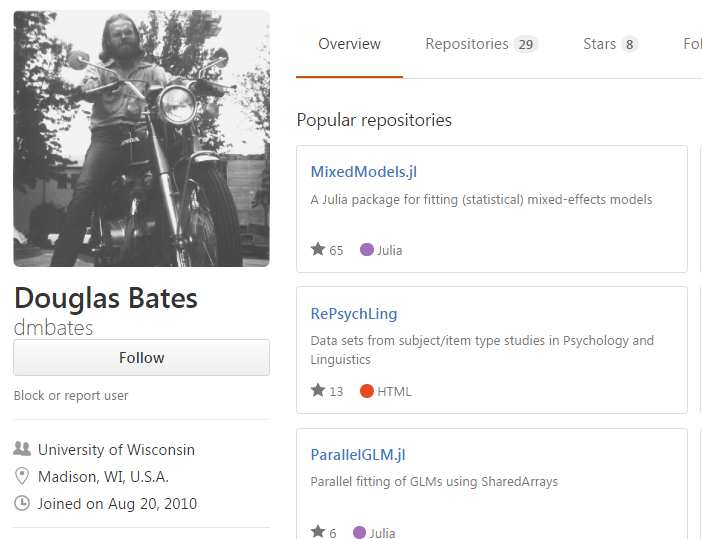
\includegraphics[width=0.99\linewidth]{images/douglasbatesgithub}

\end{figure}
\end{frame}
%================================================%
\begin{frame}[fragile]
	\begin{figure}
\centering
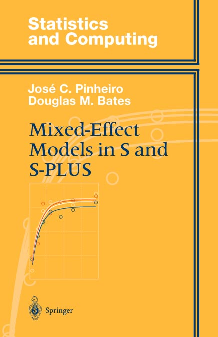
\includegraphics[width=0.50\linewidth]{images/PB-book}
\caption{}
\label{fig:PB-book}
\end{figure}
\end{frame}
%================================================%
\begin{frame}
	\begin{figure}
		\centering
		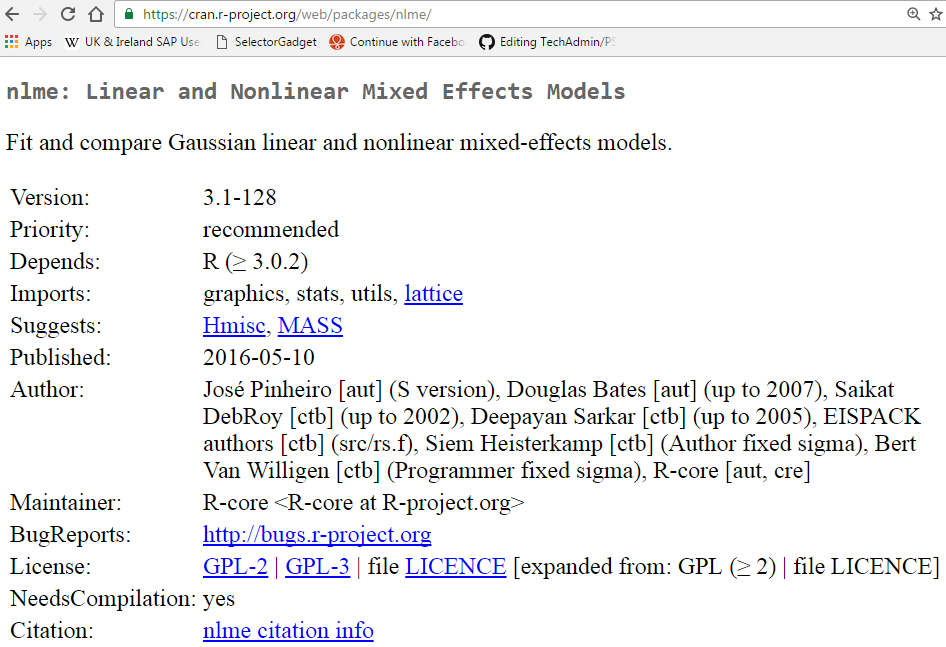
\includegraphics[width=0.97\linewidth]{images/nlmeCRAN}
	\end{figure}
\end{frame}
\begin{frame}
%=================================================%	
	\begin{figure}
\centering
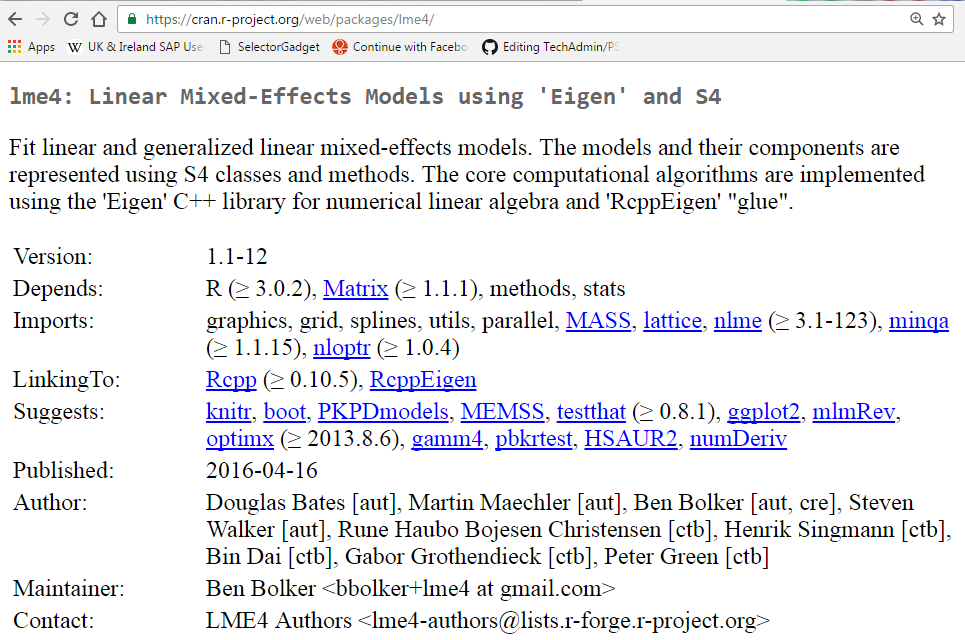
\includegraphics[width=0.97\linewidth]{images/lme4CRAN}

\end{figure}
\end{frame}
%================================================%
\begin{frame}[fragile]
	\frametitle{Statistics with Julia}
	\large
\begin{figure}
\centering
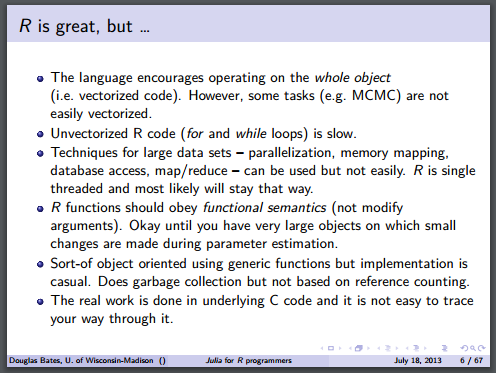
\includegraphics[width=0.98\linewidth]{images/Dougbates-R1}
\caption{}
\label{fig:Dougbates-R1}
\end{figure}




\end{frame}
%================================================%
\begin{frame}[fragile]
	\frametitle{Statistics with Julia}
	\large

\begin{figure}
	\centering
	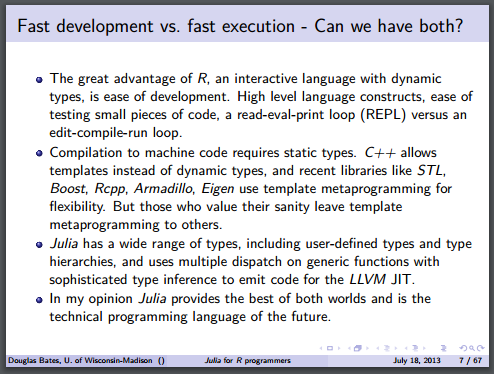
\includegraphics[width=0.98\linewidth]{images/Dougbates-R2}
	\caption{}
	\label{fig:Dougbates-R2}
\end{figure}

\end{frame}
%================================================%
\begin{frame}[fragile]
	\frametitle{Statistics with Julia}
	\large
	
	\begin{figure}
		\centering
		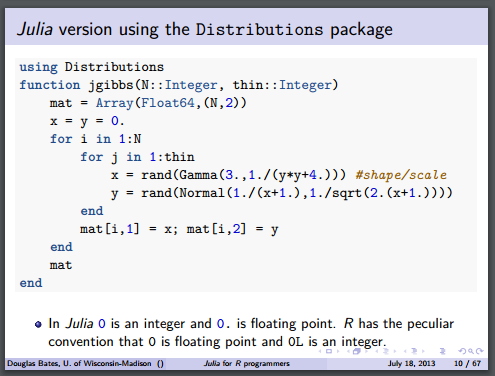
\includegraphics[width=0.98\linewidth]{images/Dougbates-R3}
		\caption{}
		\label{fig:Dougbates-R3}
	\end{figure}
	
\end{frame}
\end{document}	